\documentclass{article}
%=================================================
% Basics
%=================================================
\usepackage{fixltx2e} % Makes \( \) equation style robust, among other
                      % things. Must be the first package.


% Makes ligatured fonts searchable and copyable in pdf readers
\usepackage{cmap} % Load before fontenc 

% Always include these font encodings in your document 
% unless you have a very good reason.
\usepackage[T1]{fontenc}
\usepackage[utf8]{inputenc}

\usepackage{verbatim}

%=============
% Fonts
%=============

\usepackage{lmodern} % Improved version of computer modern
\usepackage[scale=0.88]{tgheros} % Helvetica clone for sans serif font


\newcommand\hmmax{2} % Default is 3.
\newcommand\bmmax{2} % Default is 4.

\usepackage{bm} % boldmath must be called after the package
\providecommand{\mathbold}[1]{\bm{#1}}

%=============
% AMS Packages and fonts
%=============
\usepackage{amsmath,amsbsy,amsgen,amscd,amsthm,amsfonts,amssymb} 

%=============
% Margins and paper size
%=============
\usepackage[centering,top=1.5in,bottom=1.2in,left=1.4in,right=1.4in]{geometry}
\usepackage{parskip}


%=============
% Section headings
%=============
\usepackage[sf,bf,compact]{titlesec}

%=============
% Tables and lists
%=============
\usepackage{booktabs,longtable,tabu} % Nice tables
\setlength{\tabulinesep}{1mm}
\usepackage[font=small,margin=10pt,labelfont={sf,bf},labelsep={space}]{caption}

%=============
% Code output
%=============
% \usepackage{listings}
% \usepackage{minted}




\usepackage{enumitem}
\setitemize{itemsep=0pt} 
\setenumerate{itemsep=0pt}
\setlist{labelindent=\parindent,%  % Recommended by enumitem package
  font=\sffamily}


%=============
% Hyperlink colors
%=============
\usepackage[usenames,dvipsnames]{xcolor}
\definecolor{steelblue}{HTML}{A1BDC7}
\definecolor{orange}{HTML}{D98C21}
\definecolor{silver}{HTML}{B0ABA8}
\definecolor{rust}{HTML}{B8420F}
\definecolor{seagreen}{HTML}{2E6B69}
\definecolor{joshua}{HTML}{FBDC7F}
\definecolor{darksky}{HTML}{154c79}

\colorlet{steelblue}{silver!30!white}
\colorlet{darkorange}{orange!85!black}
\colorlet{darksilver}{silver!85!black}
\colorlet{darksteelblue}{steelblue!85!black}
\colorlet{darkrust}{rust!85!black}
\colorlet{darkseagreen}{seagreen!85!black}

\usepackage{url}
\usepackage[colorlinks=true]{hyperref}
\hypersetup{linkcolor=darkrust}    
\hypersetup{citecolor=darkseagreen}      
\hypersetup{urlcolor=darksilver}     

%=============
% Microtype
%=============
\usepackage[final]{microtype} 

%=====================
% Header
%=====================
% \usepackage{fancyhdr}
% \usepackage{nopageno} % Gets rid of page number at the bottom
% \fancyhf{} % Clear header style
% \renewcommand{\headrulewidth}{0.5pt} % remove the header rule
% \pagestyle{fancy}
% \fancyhead[LE,RO]{\textsf{\small \thepage}}
% 
% \setlength{\headheight}{14pt}
%=====================
% Fix delimiters
%=====================

% Fixes \left and \right spacing issues. See discussion at
% http://tex.stackexchange.com/questions/2607/spacing-around-left-and-right
\let\originalleft\left
\let\originalright\right
\renewcommand{\left}{\mathopen{}\mathclose\bgroup\originalleft}
\renewcommand{\right}{\aftergroup\egroup\originalright}

%=================================================
% Math macros
%=================================================

%=============
% Generalities
%=============
\usepackage{mathtools}
\mathtoolsset{centercolon}  % Makes := typeset correctly for definitions

%%% Equation numbering
%\numberwithin{equation}{section} 

%%% Annotations
\newcommand{\notate}[1]{\textcolor{red}{\textbf{[#1]}}}

%==============
% Symbols
%==============
\let\oldphi\phi
\let\oldeps\epsilon

\renewcommand{\phi}{\varphi}
\renewcommand{\epsilon}{\varepsilon}
\newcommand{\eps}{\varepsilon}

%==============
% Constants
%==============

% Set constants upright
\newcommand{\cnst}[1]{\mathrm{#1}}  
\newcommand{\econst}{\mathrm{e}}

\newcommand{\zerovct}{\vct{0}} % Zero vector
\newcommand{\Id}{\mathbf{I}} % Identity matrix
\newcommand{\onemtx}{\bm{1}}
\newcommand{\zeromtx}{\bm{0}}

%==============
% Sets
%==============
\providecommand{\mathbbm}{\mathbb} % In case we don't load bbm

% Reals, complex, naturals
\newcommand{\R}{\mathbbm{R}}
\newcommand{\C}{\mathbbm{C}}
\newcommand{\K}{\mathbbm{K}}
\newcommand{\N}{\mathbbm{N}}

%==============
% Probability
%==============
\newcommand{\Prob}{\operatorname{\mathbbm{P}}}
\newcommand{\Expect}{\operatorname{\mathbb{E}}}

%==============
% Vectors and matrices 
%==============
\newcommand{\vct}[1]{\mathbold{#1}}
\newcommand{\mtx}[1]{\mathbold{#1}}

\newcommand{\mrange}{\operatorname{range}}
\newcommand{\mnull}{\operatorname{null}}



\newcommand{\eqn}[1]{\begin{equation*}#1\end{equation*}}
\newcommand{\aln}[1]{\begin{align*}#1\end{align*}}

\begin{document}

\title{CSE 6220 Homework 3}
\author{Karl Hiner, @khiner6}
\date{}
\maketitle

\section{}
Draw a 8-element bitonic sorting circuit to sort elements in non-increasing order.
Use horizontal lines for the numbers and vertical lines to denote comparison operations.
Label the comparison operations as $\uparrow$ or $\downarrow$ where the direction of the arrowhead indicates
the destination of the smaller element.
Illustrate how the input 15, 2, 7, 4, 17, 3, 9, 1 is sorted using the diagram.

\begin{figure}[htb]
  \begin{center}
  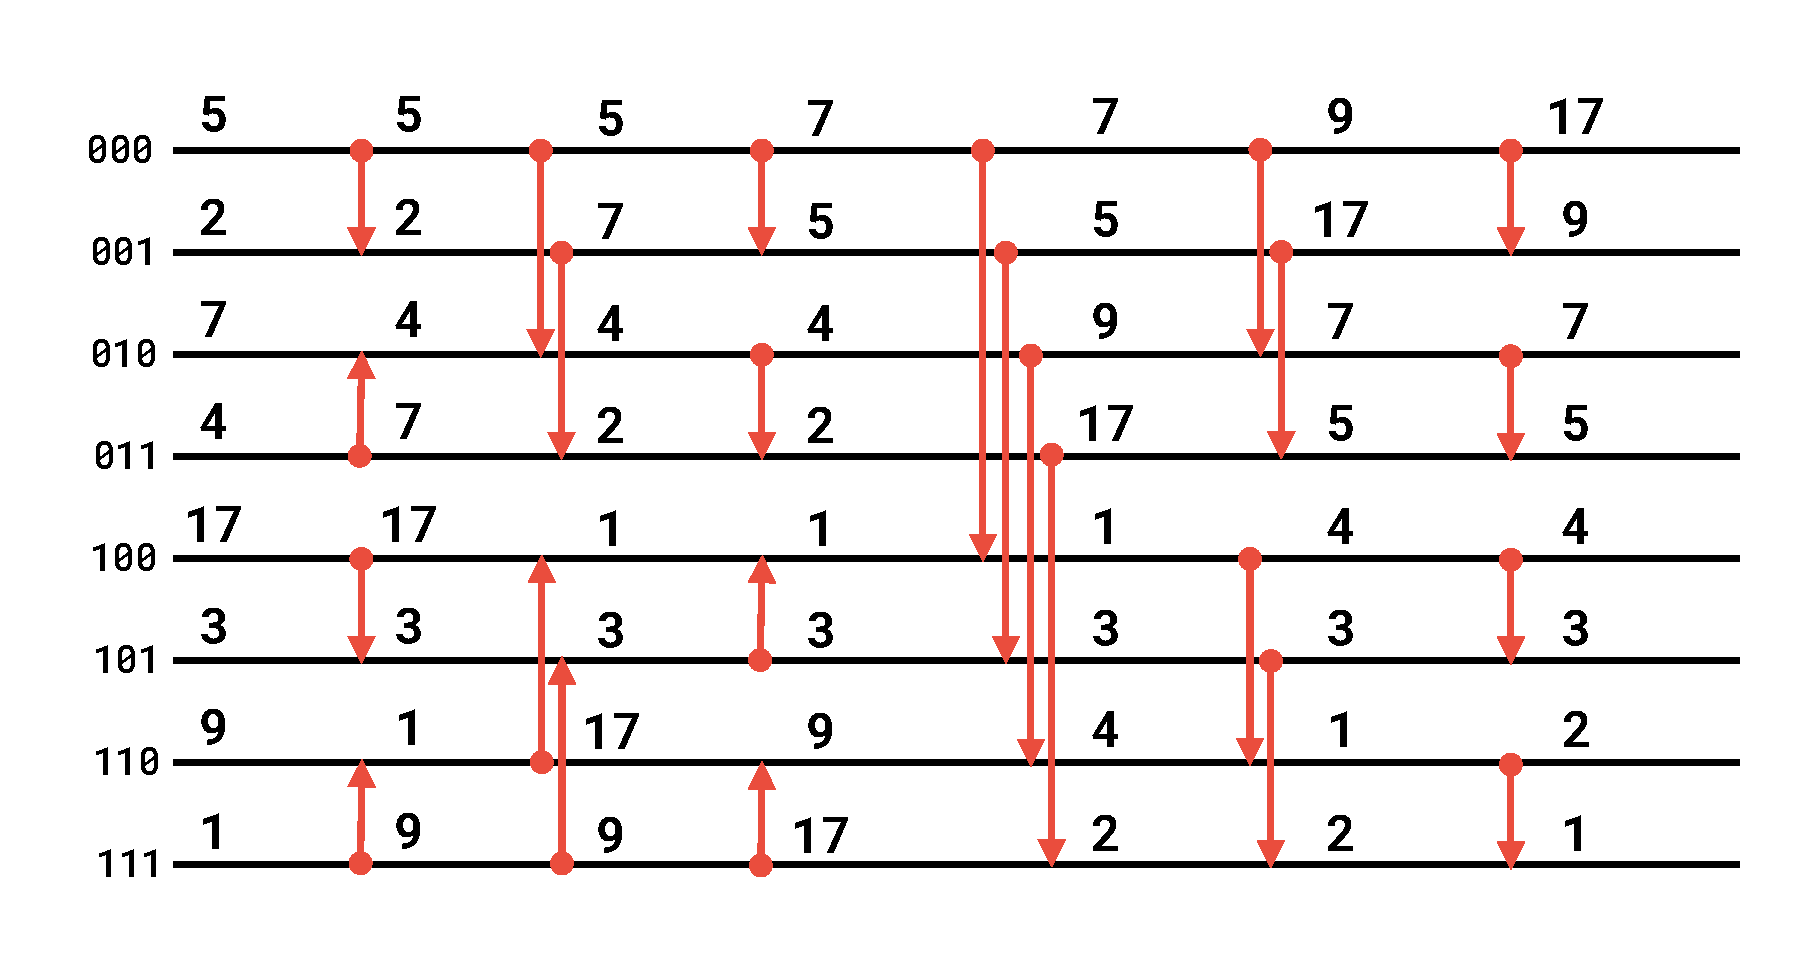
\includegraphics[width=120mm]{bitonic_sort_reversed.pdf}
  \end{center}
\end{figure}

\quad The only modification needed to the bitonic sort algorithm to sort elements in \textit{non-increasing} order, instead of \textit{non-decreasing} order, is to flip the \verb|Compare_Exchange| directions.

\section{}
The \textit{Bitonic Split} operation defined in class assumes that the bitonic sequence has
an even length.
Extend this operation to bitonic sequences of odd length.
Now, show how the bitonic sequence 5, 3, 4, 7, 10, 14, 17, 13, 8 can be converted into a sorted sequence using
repeated bitonic split operations.

\quad Here is the operation defined in class: A Bitonic Split of a bitonic sequence $l = x_0, x_1, \cdots, x_{n-1}$ is defined as a decomposition of $l$ into
\begin{itemize}
  \item $l_{min} = \min{(x_0, x_{\frac{n}{2}})}, \min{(x_1, x_{\frac{n}{2} + 1})}, \cdots, \min{(x_{\frac{n}{2} - 1}, x_{n-1})}$
  \item $l_{max} = \max{(x_0, x_{\frac{n}{2}})}, \max{(x_1, x_{\frac{n}{2} + 1})}, \cdots, \max{(x_{\frac{n}{2} - 1}, x_{n-1})}.$
\end{itemize}

One way to extend this operation to bitonic sequences of odd length is to use a similar strategy to the one we used to extend parallel prefix to non-power-of-two numbers of processors.
In that case, we kept the exact same algorithm, "pretending" that there were $p = 2^{m}$ processors, and ignored them during communication.
Similarly, we can "pretend" the given sequence $l$ has length $2m$, by appending a "dummy" element if $l$ has odd length.
Then, after completion of the split, we can remove the dummy element.

Let $\tilde{l} \equiv l + \{D\}$ refer to the sequence obtained by appending the element $D$ to the sequence $l$.
Then as long as we choose $D$ such that $\tilde{l}$ is also bitonic, after we apply the usual split operation we will have bitonic split sequences $\tilde{l}_{min}$ and $\tilde{l}_{max}$, and we will also have $\max{(\tilde{l}_{min})} \leq \min{(\tilde{l}_{max})}.$

When we later \textit{remove} the appended element $D$, we must remove it from either $\tilde{l}_{min}$ or $\tilde{l}_{max}.$
If $D$ was in $\tilde{l}_{min}$, removing it will clearly maintain $\max{\left(\tilde{l}_{min} - \{D\}\right)} \leq \max{\left(\tilde{l}_{min}\right)}$.
Likewise, removing $D$ from $\tilde{l}_{max}$ will maintain $\min{\left(\tilde{l}_{max} - \{D\}\right)} \geq \min{\left(\tilde{l}_{max}\right)}$.
So we have $\max{\left(\tilde{l}_{min} - \{D\}\right)} \leq \min{\left(\tilde{l}_{max} - \{D\}\right)}.$
Finally, note that by the definition of bitonic sequences, removing \textit{any} single element from a bitonic sequence results in another bitonic sequence.

Thus, if we append an element that produces another bitonic sequence, then perform the usual split operation on the resulting sequence, and finally remove the appended element, we maintain all properties required for the Bitonic Split operation.
A simple choice for $D$ which guarantees $\tilde{l}$ is bitonic is to \textit{duplicate the last element}.
(We could also \textit{prepend} the first element.)

Here is our algorithm:

\begin{itemize}
  \item If $l$ has length $1$ or $2$, there is nothing to do.
  \item Otherwise, if $l$ has even length greater than $2$, perform ordinary bitonic split.
  \item Otherwise, if $l = x_0, x_1, \cdots, x_{n-1},$ has odd length greater than $1$, 
  \begin{itemize}
    \item Append a new element $D = l_{n-1}$ to create $\tilde{l} =x_0, x_1, \cdots, x_{n-1}, x_{n-1}.$
    \item Perform ordinary bitonic split on $\tilde{l},$ marking the new position of the element $D$ during its compare-exchange.
    \item Create split sequences $l_{min} \equiv \tilde{l}_{min} - \{D\},\quad l_{max} \equiv \tilde{l}_{max} - \{D\}.$
  \end{itemize}
\end{itemize}

\begin{center}
  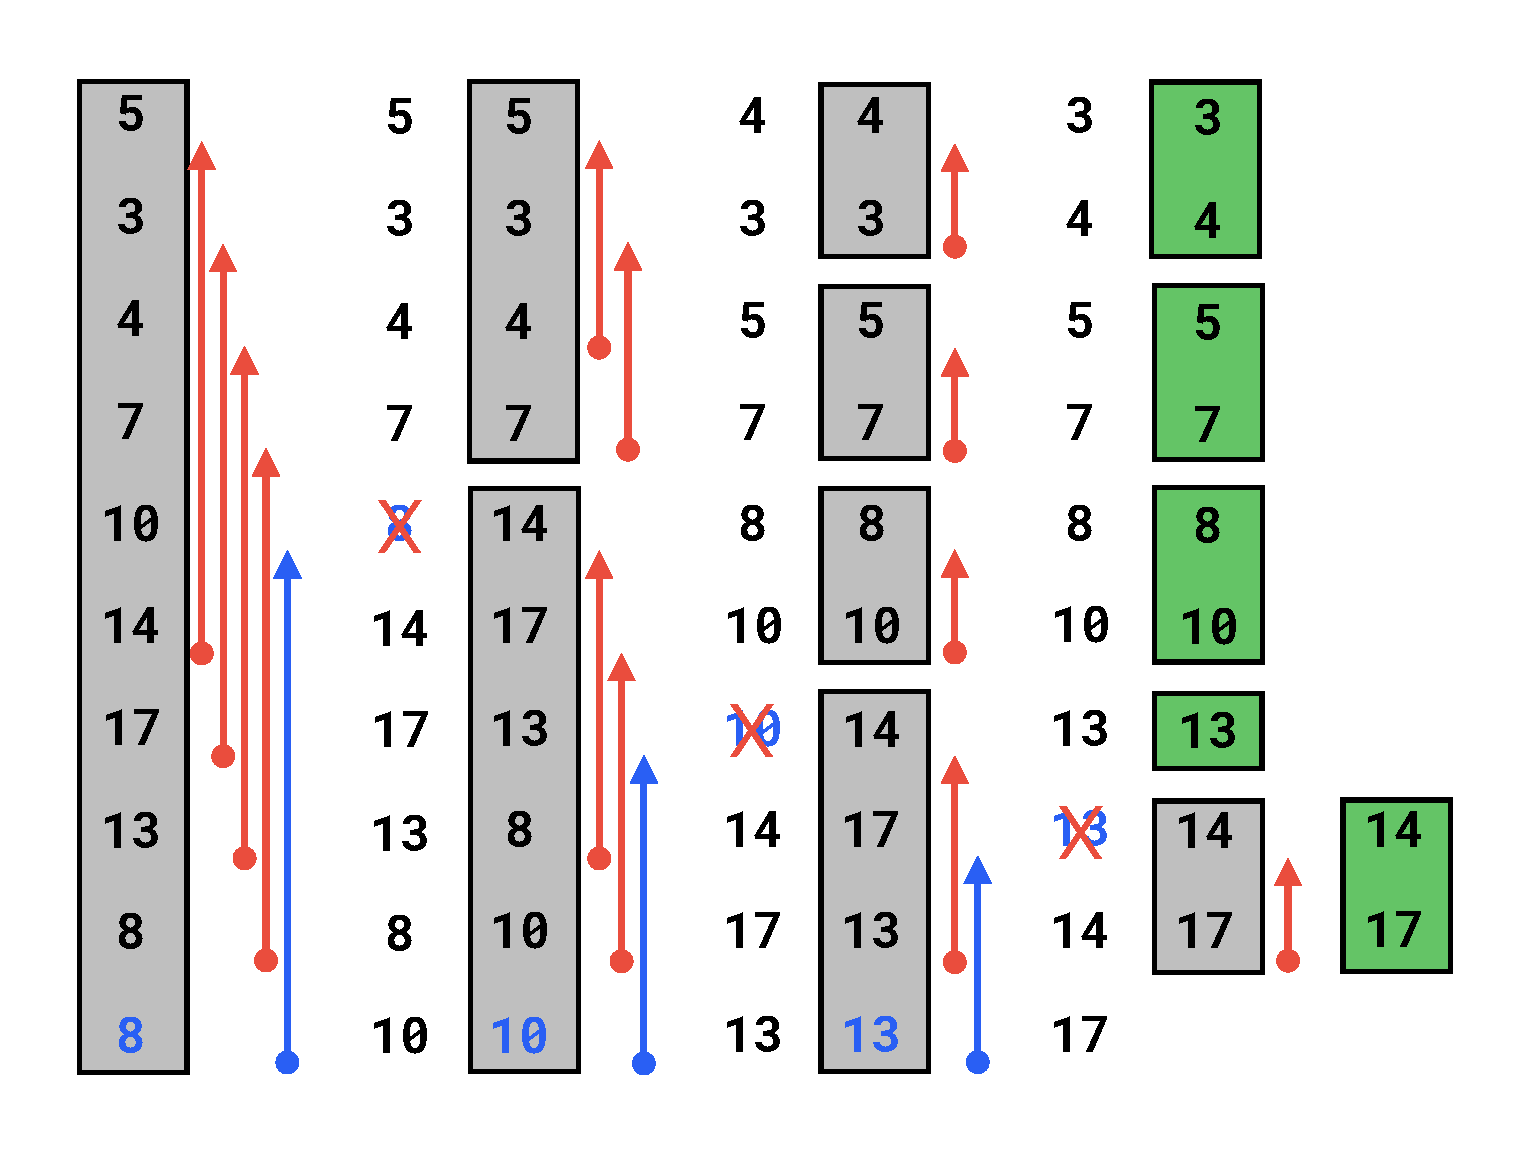
\includegraphics[width=100mm]{odd_length_bitonic_sort.pdf}
\end{center}

\section{}
Give an algorithm to merge two sorted sequences of lengths $m$ and $n$, respectively.
You may assume that the input is an array of length $m+n$ with one sequence followed by the other, distributed across processors such that each processor has a subarray of size $\frac{m+n}{p}$.
What are the computation and communication times for your algorithm?
(You may assume the use of any permutation-style communication, not necessarily hypercubic.)

\section{}
Two algorithms are designed for the All-to-all communication primitive, and have
the following runtimes:

\aln{
  \text{Algorithm 1} &:&\Theta\left(\tau\log{p} + \mu m p \log{p}\right)\\
  \text{Algorithm 2} &:&\Theta\left(\tau p + \mu m p\right)
}
Determine which algorithm runs faster asymptotically as a function of the message size.

\section{}
Consider a tree of $n$ nodes and having a bounded degree (i.e., the number of children per node is bounded by a constant).
The tree is stored in an array $A$ of size $n$.
Each node also contains the indices at which its parent and children are stored in the array.
The array is distributed among processors using block decomposition, i.e., $P_i$ contains $A[i\frac{n}{p}],A[i\frac{n}{p} + 1], \dots, A[(i + 1)\frac{n}{p} - 1].$
For each of the following operations, which communication primitive will you use and what is the runtime?

\begin{enumerate}[label=(\alph*)]
  \item Each node in the tree has $O(1)$ sized data that should be sent to its parent.
  \item Each node in the tree has $O(1)$ sized data that should be sent to all its children.
\end{enumerate}

\end{document}
